%%%%%%%%%%%%%%%%%%%%%%%%%%%%%%%%%%%%%%%%%
% NIWeek 2014 Poster by T. Reveyrand
% www.microwave.fr
% http://www.microwave.fr/LaTeX.html
% ---------------------------------------
% 
% Original template created by:
% Brian Amberg (baposter@brian-amberg.de)
%
% This template has been downloaded from:
% http://www.LaTeXTemplates.com
%
% License:
% CC BY-NC-SA 3.0 (http://creativecommons.org/licenses/by-nc-sa/3.0/)
%
%%%%%%%%%%%%%%%%%%%%%%%%%%%%%%%%%%%%%%%%%

%----------------------------------------------------------------------------------------
%   PACKAGES AND OTHER DOCUMENT CONFIGURATIONS
%----------------------------------------------------------------------------------------

\documentclass[a0paper,portrait]{baposter}

\usepackage[font=small,labelfont=bf]{caption} % Required for specifying captions to tables and figures
\usepackage{booktabs} % Horizontal rules in tables
\usepackage{relsize} % Used for making text smaller in some places

\usepackage{amsmath,amsfonts,amssymb,amsthm} % Math packages
\usepackage{eqparbox}

\usepackage{textcomp}

\usepackage{caption}
\usepackage{subcaption}
\usepackage{graphicx}

\graphicspath{{figures/}} % Directory in which figures are stored

 \definecolor{bordercol}{RGB}{40,40,40} % Border color of content boxes
 \definecolor{headercol1}{RGB}{186,215,230} % Background color for the header in the content boxes (left side)
 \definecolor{headercol2}{RGB}{120,120,120} % Background color for the header in the content boxes (right side)
 \definecolor{headerfontcol}{RGB}{0,0,0} % Text color for the header text in the content boxes
 \definecolor{boxcolor}{RGB}{210,235,250} % Background color for the content in the content boxes


\begin{document}

\background{ % Set the background to an image (background.pdf)
\begin{tikzpicture}[remember picture,overlay]
\draw (current page.north west)+(-2em,2em) node[anchor=north west]
{
\includegraphics[height=1.1\textheight]{background}};
\end{tikzpicture}
}

\begin{poster}{
grid=false,
columns=4,
borderColor=bordercol, % Border color of content boxes
headerColorOne=headercol1, % Background color for the header in the content boxes (left side)
headerColorTwo=headercol2, % Background color for the header in the content boxes (right side)
headerFontColor=headerfontcol, % Text color for the header text in the content boxes
boxColorOne=boxcolor, % Background color for the content in the content boxes
headershape=roundedright, % Specify the rounded corner in the content box headers
headerfont=\Large\sf\bf, % Font modifiers for the text in the content box headers
textborder=rectangle,
background=none,
headerborder=open, % Change to closed for a line under the content box headers
boxshade=plain
}
{
\includegraphics[width=3cm]{BiAtA2017.png}}
%
%----------------------------------------------------------------------------------------
%   TITLE AND AUTHOR NAME
%----------------------------------------------------------------------------------------
%
{ \bf  \huge {Graph Parsing Application for Bioinformatics Problems} \\  \Large \it Grammar-based approach for graph-structured data analysis} % Poster title
{\vspace{0.3em} \smaller \textbf{Semyon Grigorev$^1$}, Artem Gorokhov$^1$, Rustam Azimov$^1$ \\  % Author names
\smaller \it $^1${Saint Petersburg State University, JetBrains, St. Petersburg, Russia } \\ % Author email addresses
\smaller  {\textbf{E-mail:} semen.grigorev@jetbrains.com}}
{
\includegraphics[width=3cm]{SPbGU_Logo.png}} % University/lab logo


%----------------------------------------------------------------------------------------
%   INTRODUCTION
%----------------------------------------------------------------------------------------
\headerbox{Motivation}{name=introduction,column=0,row=0, span=2}{

Biomedical databases contain huge amounts of rich data which can be represented as a labelled graph.
In order to investigate such data, it may be useful to extract connections with specific constraints.
One natural way to provide constraints is to specify the language of paths labels which can be done by using of grammars.
For example, one can use context-free grammars with productions $\{S \rightarrow a S b; S \rightarrow \varepsilon \}$ to query paths which labels should take form of $ab; aabb; aaabbb; ...$, or, generally, should belong to the language $L = \{a^n b^n, n \geq 0\}$.
This approach is named \emph{context-free path querying} and can be applied to some problems in bioinformatics: metagenomic assemblies analysis, .

}

\headerbox{Results}{name=results,column=2,row=0, span=2}{
Tasks described above can be solved by using common technique named graph parsing --- application of classical parsing techniques for graphs; and we have some experience in this field~\cite{GraphGLL, RelaxedRNGLR, GraphParsingGPU}.
Our results solve some problems of existing approaches (such as cycles processing problem in~\cite{Earley}), and provide an ability to use GPGPU and multi-core systems for graph parsing which can be useful for huge biological data analysis.
\begin{itemize} 
\item Graph parsing framework
\vspace{-0.2cm}
\item !!!
\vspace{-0.2cm}
\item !!!
\end{itemize}
}
    
\headerbox{Future Research}{name=future,column=2,below=results, span=2}{
\begin{itemize} 
\item Currently we are working on long subsequences of 16s rRNA reconstruction from metagenomic assembly and on entities connections detection.
\vspace{-0.2cm}
\item Our aim is to present current results and also to find other applications for this techniques.
\vspace{-0.2cm}
\item Context-free compressed data processing
\end{itemize}
}

\headerbox{Context-free path querying}{name=CFParsing,span=2,column=0,row=1,below=introduction}{

\begin{center}
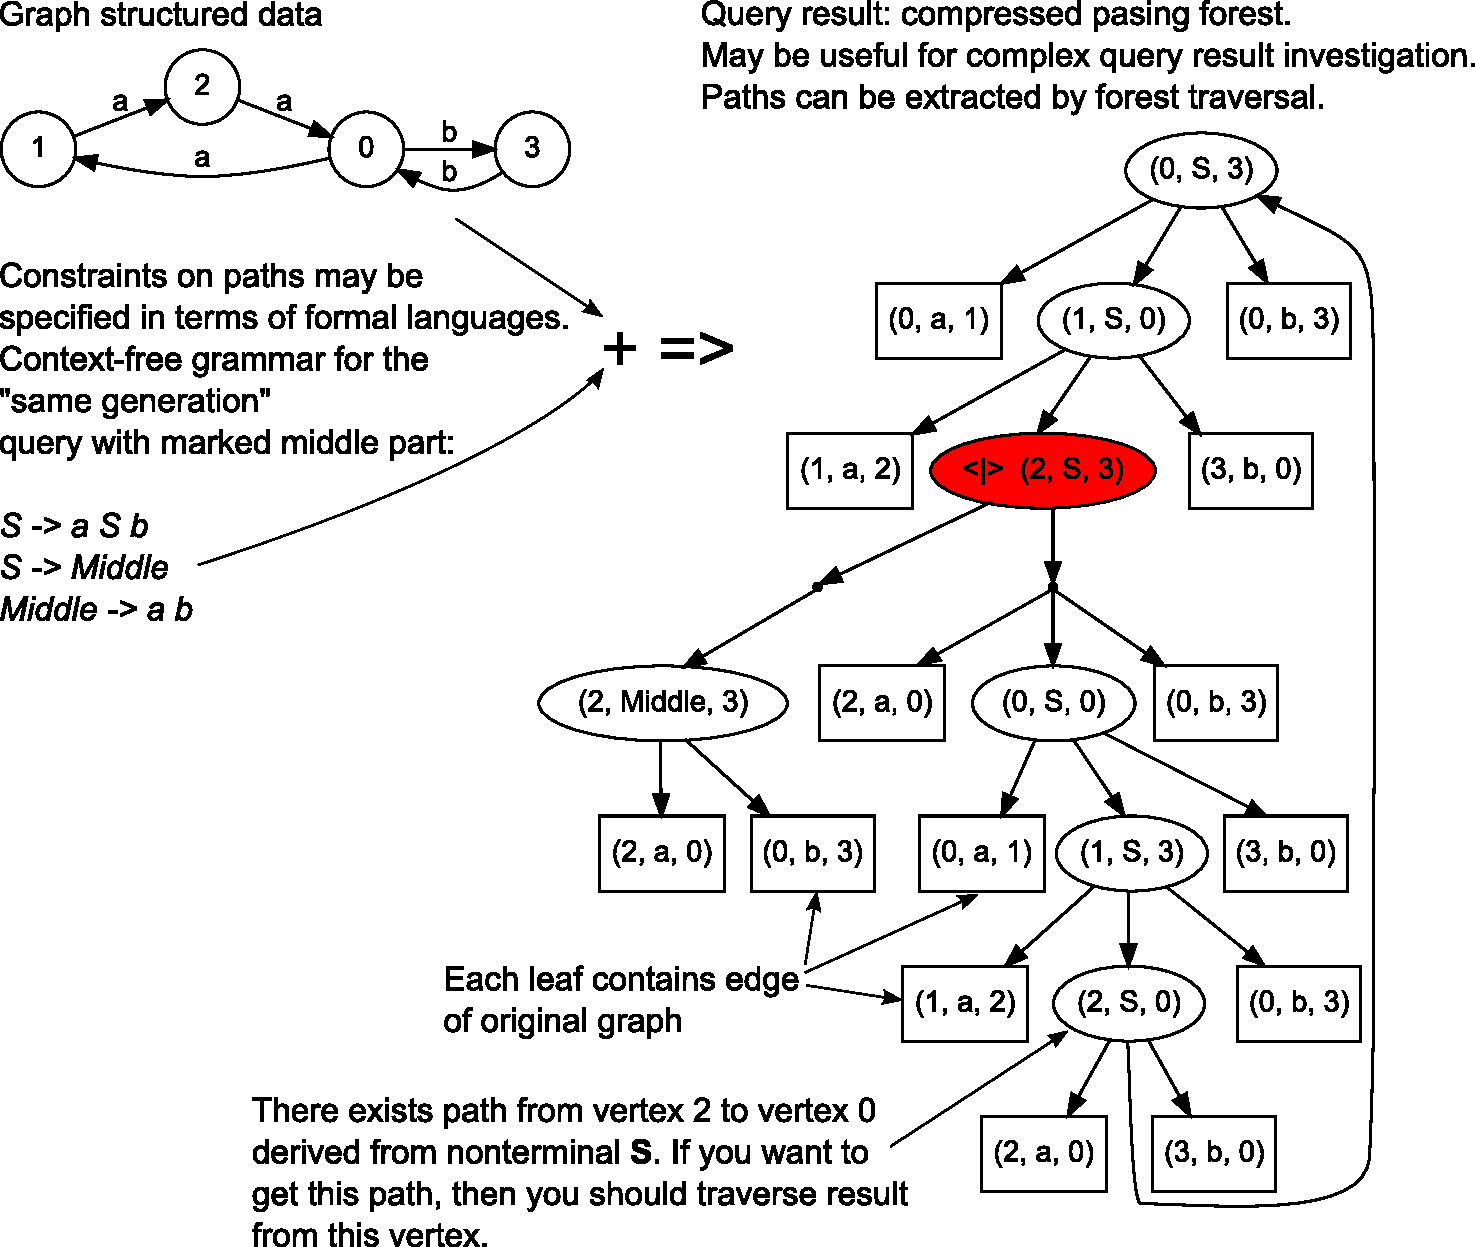
\includegraphics[width=0.9\textwidth]{AnBn_r.pdf}
\end{center}
}

\headerbox{Possible application}
{name=app1,column=0,span=2, below=CFParsing}
{ % To reduce this block to 1 column width, remove 'span=2'
One of the examples is an analysis of graphs where vertices correspond to entities and concepts such as gene or phenotype while edges represent known relationships such as ``codes for'', ``interacts with'', etc (UniProt dataset~\cite{UniProt}).
Querying paths with special constraints may shed light upon unknown before links between vertices, forming the basis for new hypotheses.
}


\headerbox{Possible application}
{name=app2,column=2,span=2, below=future}
{
Another example of graph structured data is metagenomic assemblies, and the problem is long subsequences detection and reconstruction.
Some sequences have specific secondary structure, which can be described in terms of context-free grammar, and this grammar can be used for searching and classification.
A lot of research in this area and tools are based on this approach, but most of them are only aimed at linear data processing.
Despite the existence of tools for metagenomic assemblies analysis, context-free search in graph-structured assembly is still a challenge.
\begin{center}
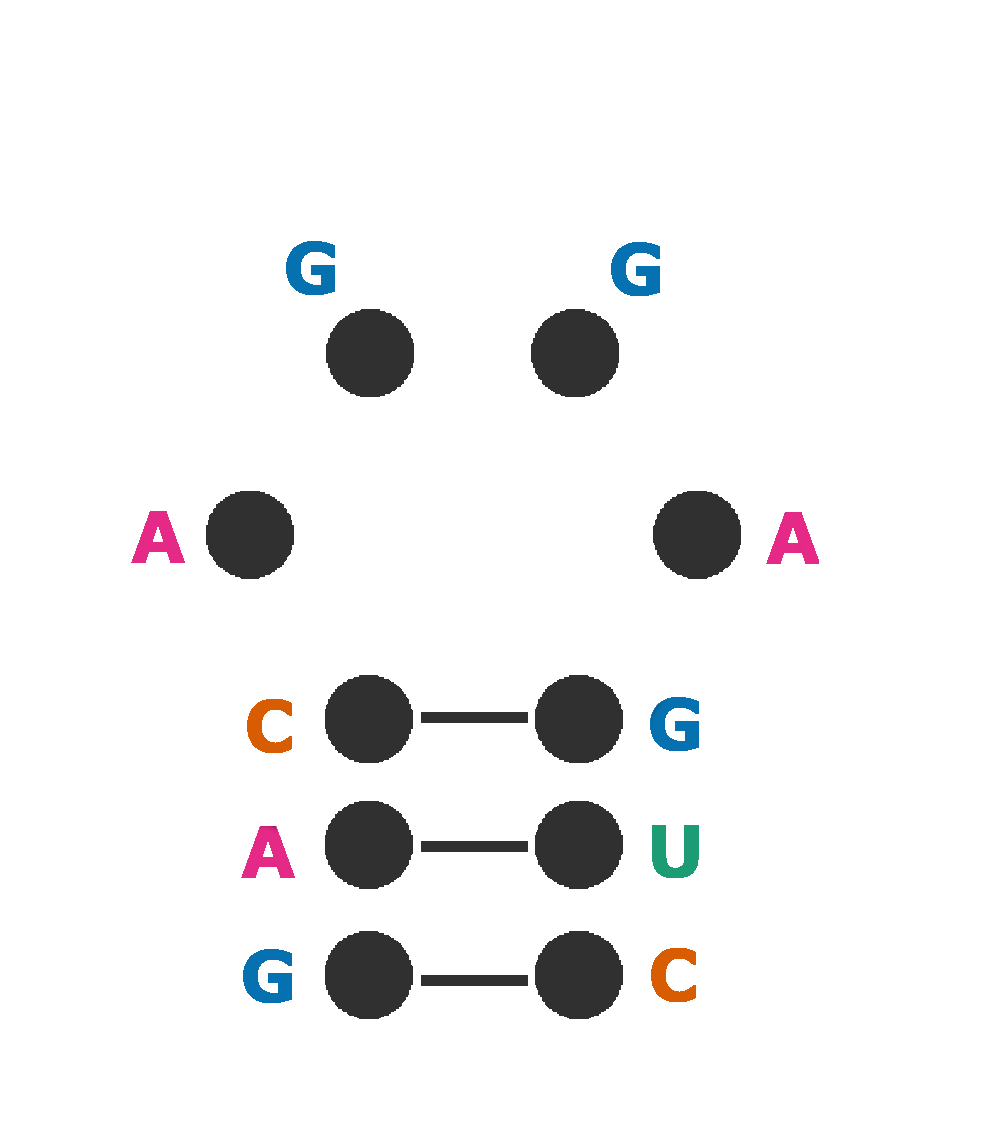
\includegraphics[width=0.4\textwidth]{RNA_small.png}
\end{center}
\begin{center}
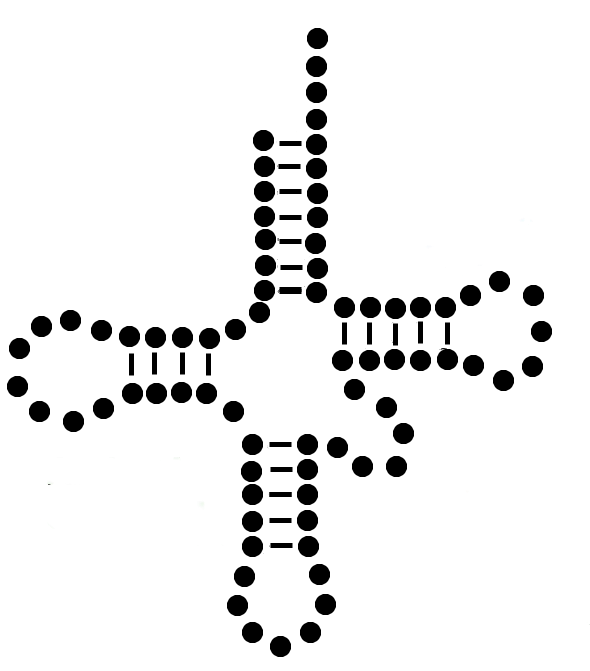
\includegraphics[width=0.4\textwidth]{tRNA.png}
\end{center}

}


%\headerbox{Possible application}
%{name=eval1,column=2,span=2, below=app2}
%{
%\begin{table}[ht]
%\centering
%\caption{Evaluation results for Query 1}

%\begin{tabular}{ | c | c | c | c | c |}
%\hline
%Ontology & \#triples & \#results & GLL(ms) & sGPU(ms) \\
%\hline 
%\hline
%skos        & 252 & 810 & 10 &  12\\
%generations & 273 & 2164 & 19 & 13\\
%travel      & 277 & 2499 & 24 & 30\\
%univ-bench  & 293 & 2540 & 25 & 15\\
%atom-primitive & 425 & 15454 & 255 & 22\\
%biomedical & 459 & 15156 & 261 & 20\\
%foaf        & 631 & 4118 & 39 & 9\\
%people-pets & 640 & 9472 & 89 & 32\\
%funding     & 1086 & 17634 & 212 & 36\\
%wine        & 1839 & 66572 & 819 & 54\\
%pizza       & 1980 & 56195 & 697 & 24\\
%$g_{1}$     & 8688 & 141072 & 1926 & 82\\
%$g_{2}$     & 14712 & 532576 & 6246 & 185\\
%$g_{3}$     & 15840 & 449560 & 7014 & 127\\
%\hline
%\end{tabular}

%\end{table}

%}




%----------------------------------------------------------------------------------------
%   REFERENCES
%----------------------------------------------------------------------------------------

\headerbox{References}{name=references,column=2,span=2,below=app2}{

\smaller % Reduce the font size in this block
\renewcommand{\section}[2]{\vskip 0.05em} % Get rid of the default "References" section title
%\nocite{*} % Insert publications even if they are not cited in the poster

\bibliographystyle{unsrt}
\bibliographystyle{IEEEtran}
\bibliography{biblio} % Use biblio.bib as the bibliography file
}


\headerbox{Acknowledgments}{name=ack,column=0,span=2,below=app1}{
This work is supported by grant from JetBrains Research.
}


\end{poster}

\end{document}